\documentclass[conference]{IEEEtran}
\IEEEoverridecommandlockouts
\usepackage{cite}
\usepackage{amsmath,amssymb,amsfonts}
\usepackage{graphicx}
\usepackage{textcomp}
\usepackage{xcolor}
\usepackage{booktabs}
\usepackage{multirow}
\usepackage{url}
\usepackage[hidelinks]{hyperref}

\def\BibTeX{{\rm B\kern-.05em{\sc i\kern-.025em b}\kern-.08em
    T\kern-.1667em\lower.7ex\hbox{E}\kern-.125emX}}

\begin{document}

\title{Provenance-Aware, Patient-Disjoint Evaluation of Ophthalmic Screening with Controlled Document Reliability\\
\large\normalfont\itshape Academic prototype --- not a medical device, not clinically validated}

\author{
\IEEEauthorblockN{Gargee Tripathi}
\IEEEauthorblockA{
\textit{Department of Computer Science and Engineering (Data Science)} \\
\textit{Manipal University Jaipur}\\{}
Jaipur, India \\
gargeetripathi123@gmail.com}
}

\maketitle

\begin{abstract}
Four-class fundus-photograph benchmarks for cataract, diabetic retinopathy,
glaucoma, and normal screening are widely reported at 95--96\% accuracy. This
paper asks how much of that number reflects retinal pathology and how much
reflects two properties of how such benchmarks are usually built: the
acquisition source an image came from, and whether the same patient's fellow
eye appears in both the training and test sets. We audit a merged four-class
benchmark built on ODIR-5K, quantify both effects, and re-evaluate a standard
image classifier under a corrected, patient-disjoint, deduplicated,
provenance-aware protocol. We find that acquisition provenance alone predicts
class with 66.7\% accuracy using no pixels, that patient-level leakage
produces no measurable inflation on a frozen linear classifier but produces a
significant $+0.022$ macro-F1 inflation (McNemar $p<0.001$) on a fine-tuned
ResNet50 --- the model that would actually be deployed --- and that this
effect grows monotonically with a model's capacity to memorize. We further
show the trained classifier does not transfer to three of four unseen
acquisition sources, and that its accuracy survives explicit age and sex
matching, indicating it is not exploiting the demographic confounds present
in the data. Building on this audit, we construct a screening prototype in
which a disease prediction is produced from the fundus image alone by
construction, while a companion referral document is used only to inform a
deferral decision. We show raw OCR confidence is a poor predictor of
extraction correctness (AUROC 0.52--0.64) but a learned estimator recovers
this signal almost completely (AUROC 0.98--0.99), that document evidence
roughly halves the area under the risk-coverage curve for deferral, and
that --- under a falsification rule fixed before the experiment --- a
learned deferral gate did not outperform two hand-written rules, a negative
result we report rather than conceal. Our contribution is empirical
throughout: an audit methodology, its quantified findings on a specific
benchmark, and a working prototype whose safety property (image-only
diagnosis) is enforced structurally rather than by convention.
\end{abstract}

\begin{IEEEkeywords}
dataset bias, patient leakage, selective prediction, ophthalmic screening,
document reliability, evaluation protocol
\end{IEEEkeywords}

\section{Introduction}

Ophthalmic screening papers built on public four-class fundus benchmarks
routinely report accuracies in the 95--96\% range using architectures such
as EfficientNetB3 and DenseNet169. These numbers are usually taken as
evidence that distinguishing cataract, diabetic retinopathy (DR), glaucoma,
and normal fundus images is close to solved by modern convolutional
networks. What such numbers measure is examined less often. A benchmark
assembled by merging several independently curated sources into one folder
per class carries structure beyond the images themselves: which camera or
export pipeline produced a file, what resolution it was saved at, and
whether a given patient's two eyes were split across train and test. None of
these properties is retinal pathology, and a sufficiently capable model can
exploit any of them.

This paper does not assert that the field's numbers are wrong. It asks,
directly and measurably: of the reported performance on a four-class
benchmark, how much is acquisition provenance, how much is patient-level
memorization, and how much survives once both are controlled for? A
screening tool that must answer on every image, regardless of its actual
certainty, is in addition not a system a clinician could reasonably deploy
--- that a system should be able to decline to answer is an argument this
paper makes, not a result it measures, and the two are kept separate
throughout.

The paper proceeds in three parts. Section~\ref{sec:audit} audits a merged
four-class benchmark and quantifies acquisition-provenance confounding and
patient-level leakage. Section~\ref{sec:results} re-evaluates a standard
classifier under a patient-disjoint, deduplicated, provenance-aware
protocol, confirming the leakage finding on a fine-tuned deployable model
rather than a linear proxy. Sections~\ref{sec:docs}--\ref{sec:triage}
present a working screening prototype in which a referral document improves
the decision to defer a case without ever influencing the diagnosis, and
show that the reliability of a machine-read document must itself be
estimated rather than assumed. Every research question below carries a
falsification criterion fixed before the corresponding experiment was run;
where an experiment produced a negative result, it is reported as such.

\begin{table}[!t]
\caption{Research questions and where each is answered}
\label{tab:rqs}
\centering
\begin{tabular}{@{}p{0.6cm}p{7cm}@{}}
\toprule
RQ & Question \\
\midrule
RQ1 & How much of reported performance is acquisition provenance? \\
RQ2 & How much is patient-level leakage and duplication? \\
RQ3 & Is raw OCR confidence a usable reliability signal for extracted clinical fields? \\
RQ4 & How does referral-document quality propagate into triage decisions? \\
RQ5 & Can document evidence improve deferral without changing the diagnosis? \\
\bottomrule
\end{tabular}
\end{table}

\section{Related Work}

This work applies existing audit and selective-prediction methodology to a
specific benchmark and a specific prototype; it does not propose a new
method in any of the areas below.

\textbf{Provenance and dataset bias.} Torralba and Efros~\cite{torralba2011}
showed that a classifier can identify which benchmark an image was drawn
from --- ``name that dataset'' --- using low-level image statistics alone.
Liu and He~\cite{liu2024decade} revisit this experiment a decade later on
modern large-scale benchmarks and show the effect persists even for
diverse, web-scale datasets. The provenance probe in this paper
(Section~\ref{sec:audit}) is a direct application of that design to a
four-class ophthalmic benchmark; it does not propose a new detection
method.

\textbf{Leakage inflation.} Tampu~\emph{et al.}~\cite{tampu2022} documented
that improper, non-patient-disjoint splitting inflates reported accuracy by
5--30 percentage points across several OCT classification benchmarks. This
paper follows the same template for fundus photography and adds a
capacity-sweep design (Section~\ref{sec:capacity}) to show that the size of
the inflation depends on whether the model being evaluated can actually
memorize a leaked example.

\textbf{Selective prediction in ophthalmology.} Leibig~\emph{et
al.}~\cite{leibig2017} and DR\textbar GRADUATE~\cite{araujo2020} established
that a diabetic-retinopathy classifier benefits from an explicit option to
abstain rather than answer on every case. This paper adopts that principle
but adds a second evidence source --- a referral document --- under the
constraint that the document must not be able to change the diagnosis,
which neither prior system needed to address since neither incorporated a
second modality.

\textbf{Reliability-weighted fusion.} Quality-aware Multimodal Fusion
(QMF)~\cite{zhang2023qmf}, Trusted Multi-view Classification
(TMC)~\cite{han2021tmc}, and MultiRetNet~\cite{she2025multiretnet} for
retinal imaging specifically motivate the deferral architecture in
Section~\ref{sec:triage}. Our instantiation of that idea is narrower:
reliability is estimated for a document-extraction pipeline rather than a
learned multimodal encoder, and the resulting comparison against
hand-written rules is reported honestly when the learned version does not
win.

\textbf{Attribution evaluation in ophthalmology.} Yavari~\emph{et
al.}~\cite{yavari2026} evaluate attribution methods in retinal imaging and
establish the standard this paper follows for its own explainability check
(Section~\ref{sec:triage}): attribution concentration and a
model-randomization sanity check, without claiming that attribution
identifies a clinical lesion absent expert annotation.

\textbf{Document information extraction.} DocILE~\cite{simsa2023docile}
established the convention of evaluating document-extraction systems on
layouts held out from development, which this paper follows directly for
its synthetic referral corpus (Section~\ref{sec:docs}): extractors are
tuned on three layouts and evaluated on three sealed ones opened only once.

\section{Data and Audit}
\label{sec:audit}

\subsection{Dataset Composition}

The evaluation dataset is the four-class subset of ODIR-5K: 5{,}058 images
from 2{,}910 patients across cataract (C), diabetic retinopathy (D),
glaucoma (G), and normal (N). Table~\ref{tab:dataset} summarizes
composition; Fig.~\ref{fig:dataset} gives the full distribution.

\begin{table}[!t]
\caption{Dataset composition}
\label{tab:dataset}
\centering
\begin{tabular}{@{}lrrrr@{}}
\toprule
Class & Images & Patients & Multi-finding & Mean age \\
\midrule
Cataract & 293 & 203 & 10.6\% & 66.8 \\
DR & 1{,}608 & 1{,}027 & 13.9\% & 55.7 \\
Glaucoma & 284 & 182 & 23.2\% & 63.0 \\
Normal & 2{,}873 & 1{,}852 & 2.0\% & 57.2 \\
\bottomrule
\end{tabular}
\end{table}

\begin{figure}[!t]
\centering
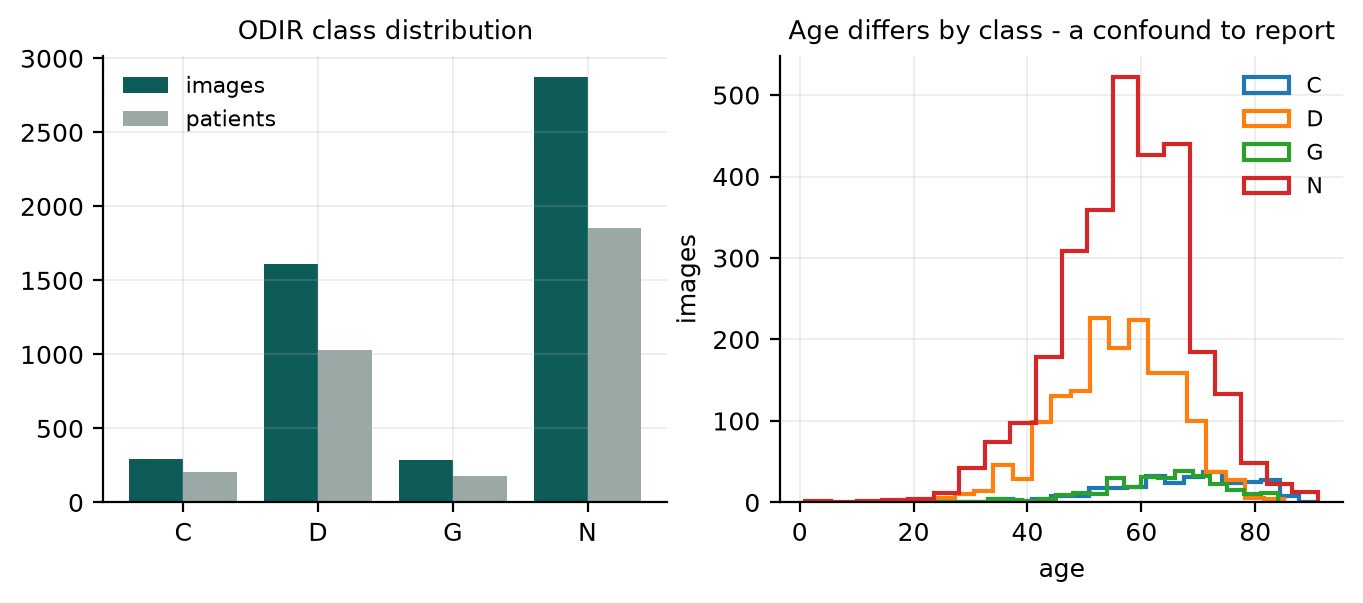
\includegraphics[width=0.9\linewidth]{../figures/fig09_dataset_composition.png}
\caption{Dataset composition by class and acquisition source.}
\label{fig:dataset}
\end{figure}

Of 2{,}910 patients, 2{,}148 contribute both eyes, which is the structural
precondition for patient-level leakage: if eyes rather than patients are
the unit of splitting, a model can encounter one eye at training time and
the fellow eye at test time. 354 patients carry different diagnoses in each
eye, so splitting is performed by patient while stratification for class
balance is performed at eye level. The corpus spans 91 distinct image
resolutions with no EXIF metadata, meaning acquisition source cannot be
read from a clean field and must instead be inferred
(Section~\ref{sec:provenance}).

Two confounds are reported here rather than deferred to a limitations
section, because Section~\ref{sec:demographics} tests them directly:
cataract patients average approximately 11 years older than
diabetic-retinopathy patients, sex distribution differs by class, and
23.2\% of glaucoma-labelled rows name a second condition in the original
annotation. ODIR is less confounded than a naively merged benchmark, but it
is not confound-free.

\subsection{Provenance Audit}
\label{sec:provenance}

Acquisition source was assigned from file properties alone --- extension,
resolution, and pixel-level export artifacts --- never from the class
folder a file was drawn from, since labelling source from class would make
any downstream probe circular. Three probes were run.

E0a predicted class from file metadata only, with no pixel content: a
majority-class baseline of 26.0\% rose to \textbf{66.7\%}. Every
diabetic-retinopathy image in this benchmark is a \texttt{.jpeg} file and
no other class contains a \texttt{.jpeg}, making file extension alone a
perfect DR detector independent of image content.

E0b predicted acquisition source from FOV-normalized pixels
($0.398\rightarrow0.749$), and E0c-i predicted source from image geometry
alone ($0.398\rightarrow0.702$): source leaves a detectable signature even
after cropping to the retinal field of view and even when only crop shape
is available.

E0c-ii, the anti-circularity control, held source constant and asked
whether class could still be predicted from pixels within a single source.
If provenance were doing all the work, this signal should vanish once
source is fixed.

\begin{table}[!t]
\caption{Anti-circularity control (E0c-ii)}
\label{tab:e0c}
\centering
\begin{tabular}{@{}lrrrr@{}}
\toprule
Source & $n$ & Baseline & Within-source & Lift \\
\midrule
\texttt{odir\_jpg512} & 1{,}678 & 0.640 & 0.644 & +0.004 \\
\texttt{crop\_jpg256} & 1{,}240 & 0.516 & 0.736 & +0.219 \\
\texttt{png\_highres} & 201 & 0.497 & 0.781 & +0.284 \\
\bottomrule
\end{tabular}
\end{table}

The result is asymmetric, and both halves are reported. Within
\texttt{odir\_jpg512} --- the source containing the DR and normal classes
--- the signal essentially vanishes (+0.004), consistent with file
extension having already explained nearly all separable variance for those
two classes. Within \texttt{crop\_jpg256} and \texttt{png\_highres} ---
sources split roughly evenly between cataract and glaucoma --- a real
signal survives (+0.219 and +0.284), indicating the
cataract-versus-glaucoma distinction is not purely a provenance artifact.
\textbf{Provenance explains the diabetic retinopathy and normal classes
almost entirely, and comparatively little of the cataract/glaucoma
separation.} Fig.~\ref{fig:heatmap} and Fig.~\ref{fig:probes} carry this
finding visually.

\begin{figure}[!t]
\centering
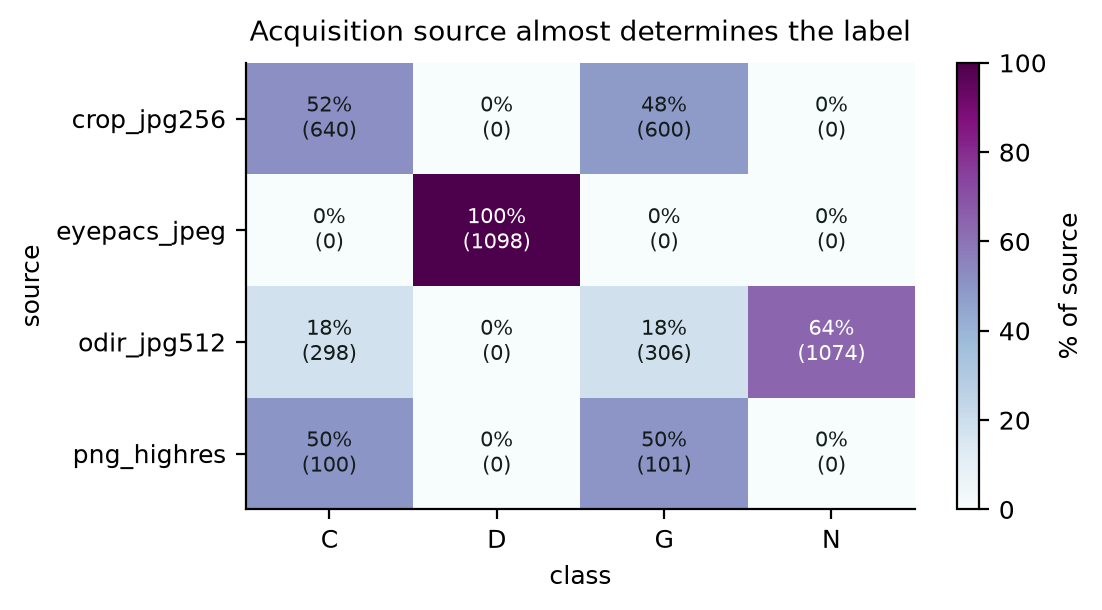
\includegraphics[width=0.9\linewidth]{../figures/fig01_provenance_heatmap.png}
\caption{Source $\times$ class heatmap.}
\label{fig:heatmap}
\end{figure}

\begin{figure}[!t]
\centering
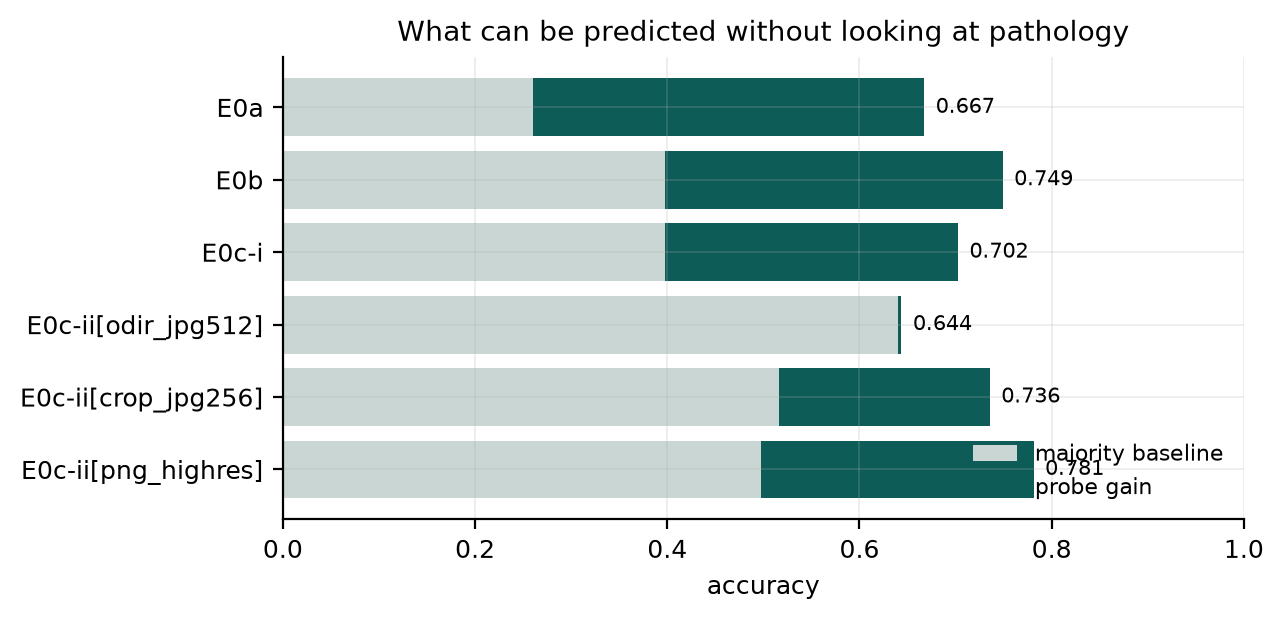
\includegraphics[width=0.9\linewidth]{../figures/fig02_provenance_probes.png}
\caption{Provenance probe comparison (E0a/E0b/E0c).}
\label{fig:probes}
\end{figure}

\subsection{Deduplication}

Two candidate detectors were evaluated against a ground truth of 1{,}654
known duplicate pairs. An ImageNet ResNet50 embedding, compared by cosine
similarity, was tried first and \textbf{failed}: at an operating threshold
of 0.999 it recovered \textbf{0\%} of known duplicates, since fundus images
are visually homogeneous to begin with and true duplicates differ by a
substantial downscale that ImageNet features are not invariant to. An
FOV-normalized $64\times64$ pixel fingerprint recovers \textbf{97\%} of the
same ground truth at 0.99 precision and is used throughout the rest of this
paper (Fig.~\ref{fig:dedup}).

\begin{figure}[!t]
\centering
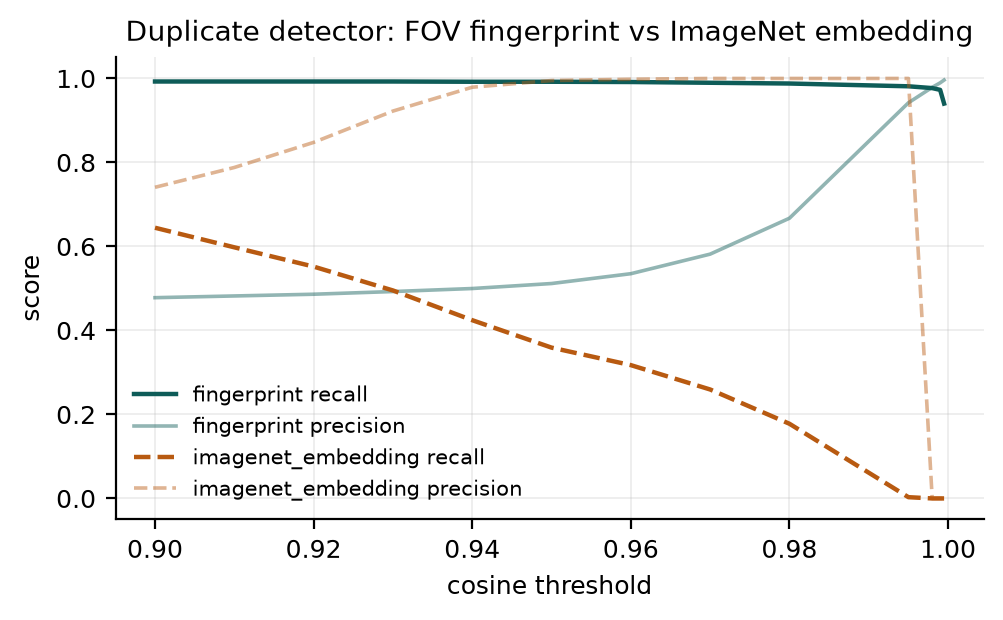
\includegraphics[width=0.9\linewidth]{../figures/fig04_duplicate_calibration.png}
\caption{Duplicate-detector calibration: rejected embedding method vs.\ FOV fingerprint.}
\label{fig:dedup}
\end{figure}

The detector's threshold required a correction after an initial
miscalibration: calibrating on a synthetic balanced sample suggested 0.98
was safe, but applied to the true search space (positive rate on the order
of one in a million pairs) it returned 26{,}634 false-positive pairs,
chaining into duplicate clusters covering 37\% of the dataset. Recalibrating
against hard negatives drawn from the real search space gave the 0.999
operating point reported above. Within ODIR, this detector found 2
duplicate groups ($5{,}058\rightarrow5{,}056$ images); across the two
benchmarks, 1{,}626 merged-benchmark images were identified as ODIR copies
and excluded from the cross-source transfer evaluation
(Section~\ref{sec:transfer}).

\section{Results}
\label{sec:results}

\subsection{Protocol Ladder: Patient Leakage on a Frozen Classifier}

Holding a frozen-ResNet50-features-plus-logistic-head model fixed, four
splitting protocols were compared.

\begin{table}[!t]
\caption{Protocol ladder, frozen features}
\label{tab:ladder}
\centering
\begin{tabular}{@{}lrrr@{}}
\toprule
Rung & $n$ & Macro-F1 & 95\% CI \\
\midrule
Image-level & 5{,}058 & 0.5496 & [0.5308, 0.5677] \\
Patient-disjoint & 5{,}058 & 0.5444 & [0.5248, 0.5622] \\
+ Dedup & 5{,}056 & 0.5476 & [0.5282, 0.5675] \\
Provenance-controlled & 1{,}535 & 0.5048 & [0.4735, 0.5383] \\
\bottomrule
\end{tabular}
\end{table}

No rung differs significantly from any other (McNemar $p\in[0.14,0.75]$;
all confidence intervals overlap; Fig.~\ref{fig:ladder}). Read alone, this
falsifies the hypothesis that patient leakage inflates accuracy on this
benchmark. It is reported as a lower bound rather than a conclusion,
because a frozen linear head has essentially no capacity to memorize a
specific training example --- and leakage inflation specifically requires
memorization.

\begin{figure}[!t]
\centering
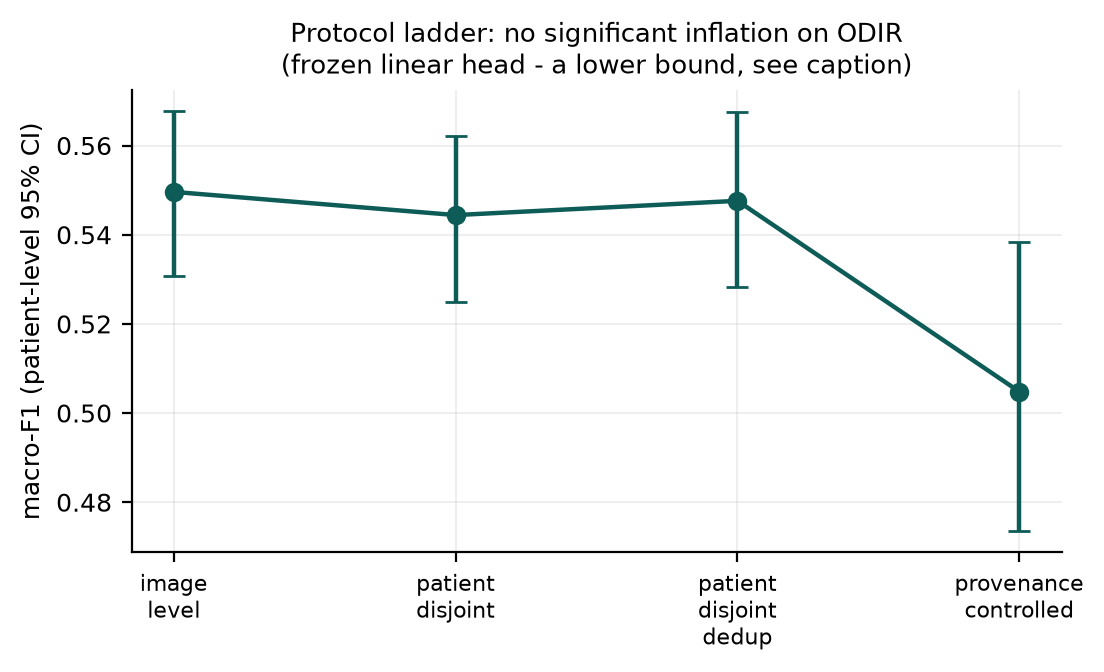
\includegraphics[width=0.9\linewidth]{../figures/fig03_protocol_ladder.png}
\caption{Protocol ladder across four splitting rungs.}
\label{fig:ladder}
\end{figure}

\subsection{Capacity Ladder: Does Inflation Require Memorization?}
\label{sec:capacity}

Holding features and splits fixed, model capacity was swept from a
logistic head up to a pure 1-nearest-neighbor (1-NN) retriever, which
recalls a leaked fellow-eye example by construction whenever one is present
in the training set.

\begin{table}[!t]
\caption{Leakage inflation vs.\ model capacity}
\label{tab:capacity}
\centering
\begin{tabular}{@{}lccc@{}}
\toprule
Model & Capacity & Inflation & McNemar $p$ \\
\midrule
Logistic & none & $+0.0052$ & 0.7467 \\
MLP & low & $+0.0274$ & 0.2006 \\
5-NN & moderate & $+0.0207$ & 0.00065 \\
1-NN & pure memorizer & $+0.0453$ & $\sim$0 \\
\bottomrule
\end{tabular}
\end{table}

Inflation increases monotonically with capacity and becomes statistically
significant once the model can meaningfully memorize (5-NN, 1-NN). This
corrects the interpretation of the protocol ladder: the earlier null result
was an artifact of testing an architecture that structurally cannot exploit
patient leakage, not evidence the benchmark is free of it
(Fig.~\ref{fig:capacity}).

\subsection{Confirmation on a Fine-Tuned, Deployable Model}

To confirm the mechanism on a model that would actually be deployed, a
ResNet50 was fine-tuned end-to-end (8 epochs, seed 42, $384\times384$
input) on a GPU, on the image-level and patient-disjoint-deduplicated
rungs.

\begin{table}[!t]
\caption{Fine-tuned confirmation (E3)}
\label{tab:e3}
\centering
\begin{tabular}{@{}lrrr@{}}
\toprule
Rung & $n$ & Macro-F1 & 95\% CI \\
\midrule
Image-level (leaky) & 5{,}058 & 0.6797 & [0.6611, 0.6967] \\
Patient-disjoint + dedup & 5{,}056 & 0.6579 & [0.6393, 0.6768] \\
\bottomrule
\end{tabular}
\end{table}

Inflation: $\mathbf{+0.0218}$ macro-F1 (McNemar $p=0.0006825$, 886
discordant predictions across 5{,}056 paired test cases).

\begin{table}[!t]
\caption{Inflation by capacity, including fine-tuned confirmation}
\label{tab:e3capacity}
\centering
\begin{tabular}{@{}lccc@{}}
\toprule
Model & Capacity & Inflation & $p$ \\
\midrule
Logistic & none & $+0.0052$ & 0.75 \\
\textbf{Fine-tuned ResNet50} & \textbf{realistic} & $\mathbf{+0.0218}$ & $\mathbf{0.0007}$ \\
1-NN retriever & pure & $+0.0453$ & $\sim$0 \\
\bottomrule
\end{tabular}
\end{table}

\begin{figure}[!t]
\centering
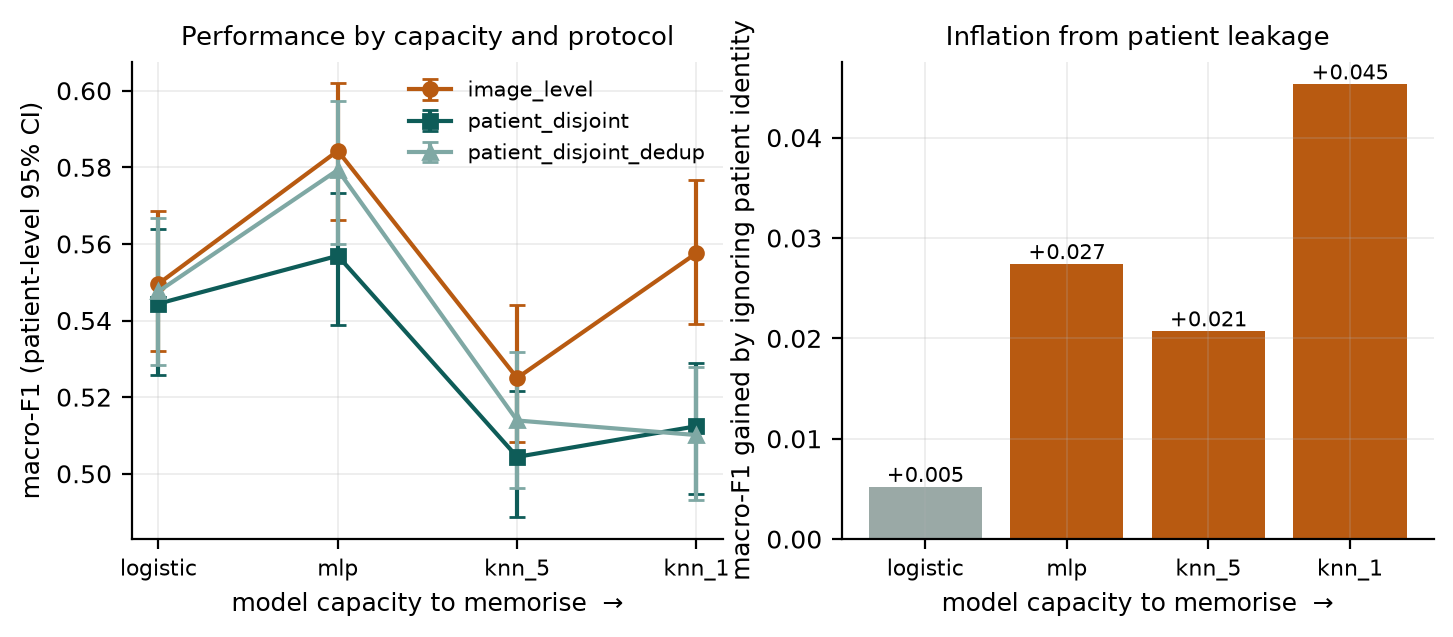
\includegraphics[width=0.9\linewidth]{../figures/fig10_capacity_ladder.png}
\caption{Capacity ladder, including the fine-tuned ResNet50 confirmation.}
\label{fig:capacity}
\end{figure}

The pattern remains monotonic in capacity and is now significant on the
model a screening application would actually use. This upgrades the claim
from a proxy-model demonstration to a confirmed property of a deployable
classifier: patient-disjoint splitting matters, and matters more as model
capacity increases --- precisely the direction the field's architectures
are moving. The result should be read as confirmatory rather than
exhaustively validated: it reflects one random seed and one backbone
trained for eight epochs, and the seed-stability treatment
(Section~\ref{sec:seeds}) was not repeated for this fine-tuned run.

\subsection{Cross-Source Transfer}
\label{sec:transfer}

The frozen-feature model trained on the 5{,}056 deduplicated ODIR images
was evaluated on merged-benchmark images from four acquisition sources,
after excluding the 1{,}626 confirmed ODIR copies, so no test image had
been seen during training.

\begin{table}[!t]
\caption{Cross-source transfer}
\label{tab:transfer}
\centering
\begin{tabular}{@{}lrrrr@{}}
\toprule
Source & $n$ & Classes & Majority acc. & Model acc. \\
\midrule
\texttt{crop\_jpg256} & 1{,}223 & C, G & 0.517 & 0.330 \\
\texttt{eyepacs\_jpeg} & 1{,}098 & D & 1.000 & 0.297 \\
\texttt{odir\_jpg512} & 69 & C, G, N & 0.449 & 0.507 \\
\texttt{png\_highres} & 201 & C, G & 0.502 & 0.104 \\
\bottomrule
\end{tabular}
\end{table}

On three of four unseen sources, model accuracy falls below simply guessing
the majority class for that source (Fig.~\ref{fig:transfer}). Because each
source is class-restricted --- itself a symptom of the provenance confound
--- results are reported per source rather than pooled. Two caveats apply:
the in-domain model is itself relatively weak (macro-F1 0.55 on frozen
features), so part of this failure reflects model quality rather than a
domain gap specifically; and this measures transfer under a documented,
discrete change of acquisition source, not generalization in an unqualified
sense.

\begin{figure}[!t]
\centering
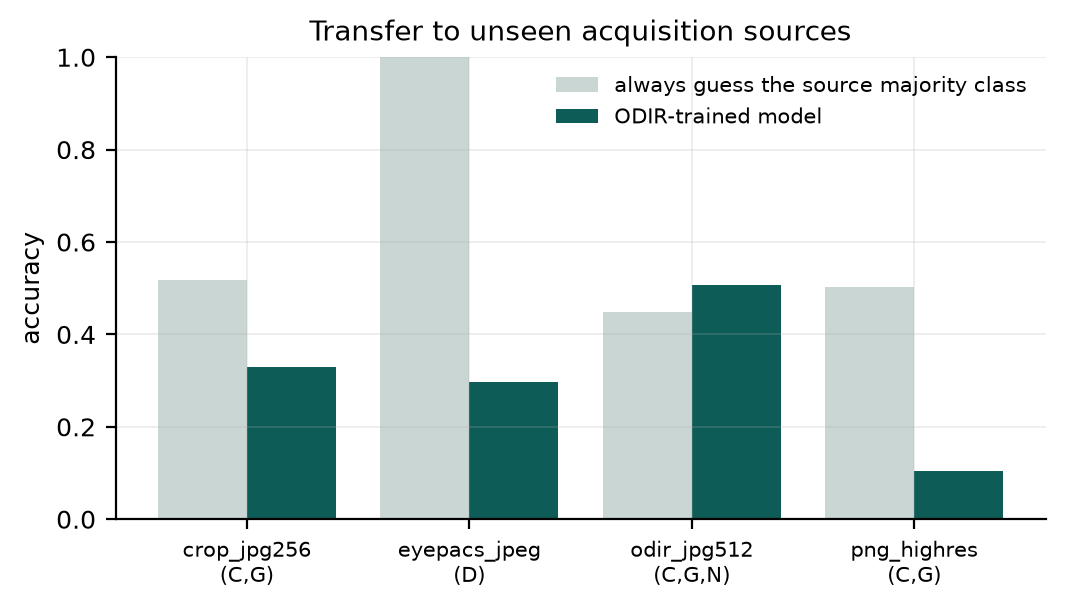
\includegraphics[width=0.9\linewidth]{../figures/fig11_cross_source_transfer.png}
\caption{Cross-source transfer to four unseen acquisition sources.}
\label{fig:transfer}
\end{figure}

\subsection{Disease Detector or Demographics Detector?}
\label{sec:demographics}

Because convolutional networks can read age and sex from fundus
photographs, the demographic confound documented in
Section~\ref{sec:audit} was tested directly rather than only disclosed. A
classifier given age and sex alone, with no image, scored 0.556 accuracy
against a 0.568 majority-class baseline (macro-F1 0.2531) ---
\textbf{worse} than always guessing the majority class.

\begin{table}[!t]
\caption{Image-model performance under demographic controls}
\label{tab:demog}
\centering
\begin{tabular}{@{}lrrrr@{}}
\toprule
Condition & $n$ & Macro-F1 & 95\% CI & Cataract AUROC \\
\midrule
Unrestricted & 5{,}056 & 0.5476 & [0.528, 0.567] & 0.9462 \\
Age-matched & 964 & 0.5385 & [0.503, 0.572] & 0.9414 \\
Sex-matched & 972 & 0.5302 & [0.500, 0.562] & 0.9406 \\
Multi-finding removed & 4{,}679 & 0.5478 & [0.526, 0.568] & 0.9560 \\
\bottomrule
\end{tabular}
\end{table}

Matching was performed by downsampling within strata, closing the
demographic route without reweighting or modelling assumptions
(Fig.~\ref{fig:confound}). Every confidence interval under a control
overlaps the unrestricted interval, and cataract-versus-rest AUROC remains
near 0.94 throughout. \textbf{The demographic confound is real in the data,
but it is not what the image model is using} --- the strongest single piece
of evidence in this paper that classifier accuracy reflects retinal content
rather than a shortcut.

\begin{figure}[!t]
\centering
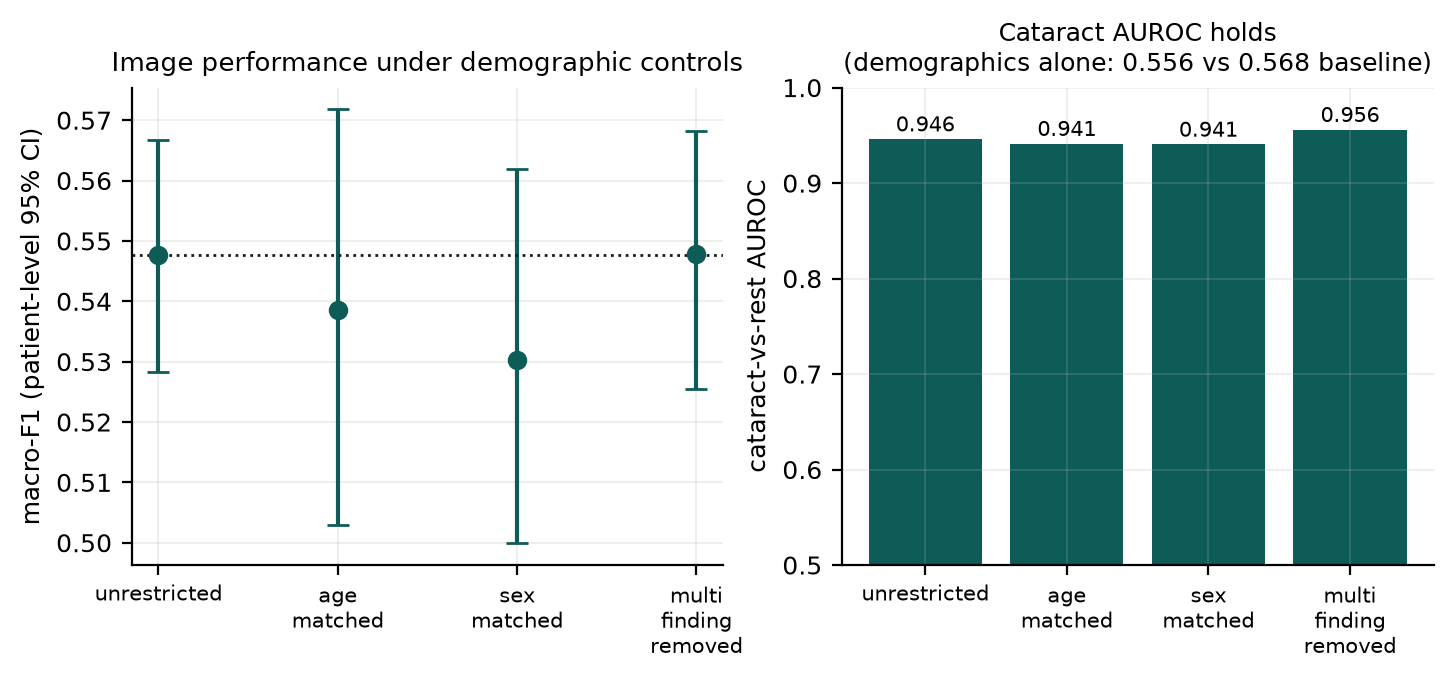
\includegraphics[width=0.9\linewidth]{../figures/fig13_confound_sensitivity.png}
\caption{Model performance under age/sex matching.}
\label{fig:confound}
\end{figure}

\subsection{Seed Stability and Multiple Comparisons}
\label{sec:seeds}

Because a finding that holds under only one random split is not a finding,
the leakage comparison was re-run under three independent split seeds (42,
7, 2024).

\begin{table}[!t]
\caption{Seed stability}
\label{tab:seeds}
\centering
\begin{tabular}{@{}lrrl@{}}
\toprule
Model & Mean inflation & sd & Range across seeds \\
\midrule
1-NN & $+0.0453$ & 0.0027 & [$+0.0434$, $+0.0484$] \\
Logistic & $-0.0031$ & 0.0085 & [$-0.0126$, $+0.0038$] \\
\bottomrule
\end{tabular}
\end{table}

The memorizer's effect is large, tightly reproducible, and significant at
every seed (Fig.~\ref{fig:seedstab}). The logistic head's effect is small,
noisy, and \textbf{changes sign between seeds} --- a direct illustration
that this effect is statistical noise rather than a real property of the
leakage mechanism at low model capacity. Because this study performs 13
paired hypothesis tests, a Holm--Bonferroni correction was applied across
the full family at $\alpha=0.05$. Five of thirteen tests survive
correction, and all five are memorization-based results. One test in
particular, \emph{leakage[logistic, seed 7]}, had an uncorrected
$p=0.037$ and a \emph{negative} effect direction --- it would have been
reported as significant without correction, and would have been wrong.
This case is the concrete justification for applying the correction.

\begin{figure}[!t]
\centering
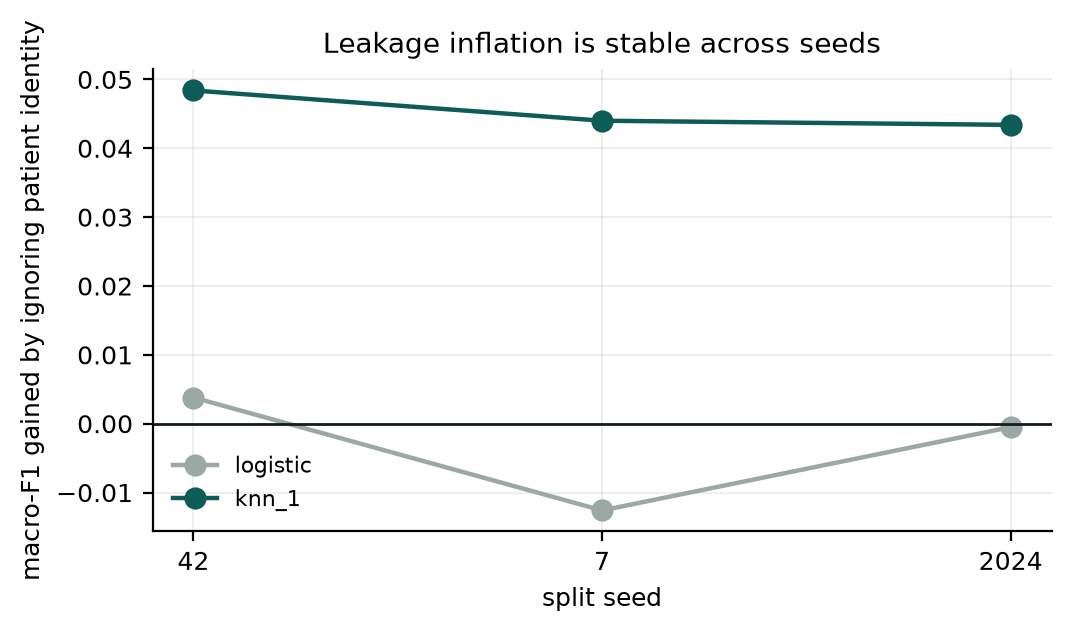
\includegraphics[width=0.9\linewidth]{../figures/fig14_seed_stability.png}
\caption{Leakage inflation across three random split seeds.}
\label{fig:seedstab}
\end{figure}

\section{Document Processing}
\label{sec:docs}

\subsection{Corpus and Extraction}

Because no suitable public de-identified ophthalmic referral corpus was
located --- a search that is recorded here rather than silently
substituted --- a synthetic corpus of 360 referral documents was generated
across six visual layouts (A--F). Two extraction methods were developed and
tuned using only layouts A--C; layouts D--F were sealed and opened exactly
once, after both extractors were frozen, following the held-out-layout
convention established by DocILE~\cite{simsa2023docile}.

\begin{table}[!t]
\caption{Extraction performance}
\label{tab:extraction}
\centering
\begin{tabular}{@{}llrrrr@{}}
\toprule
Extractor & Split & Prec. & Rec. & F1 & Exact \\
\midrule
E1 & dev & 0.696 & 0.534 & 0.604 & 0.568 \\
E1 & sealed & 0.726 & 0.235 & 0.355 & 0.297 \\
E2 & dev & 0.687 & 0.679 & 0.683 & 0.691 \\
E2 & sealed & 0.563 & 0.430 & 0.488 & 0.453 \\
\bottomrule
\end{tabular}
\end{table}

Both extractors degrade on sealed layouts relative to development layouts
(Fig.~\ref{fig:extraction}), which is expected of any layout-sensitive
extraction pipeline and motivates estimating extraction reliability rather
than assuming it (Section~\ref{sec:reliability}). Every number in this
section carries its synthetic-data caveat: this is a technical evaluation
under controlled degradation, not a clinical validation.

\begin{figure}[!t]
\centering
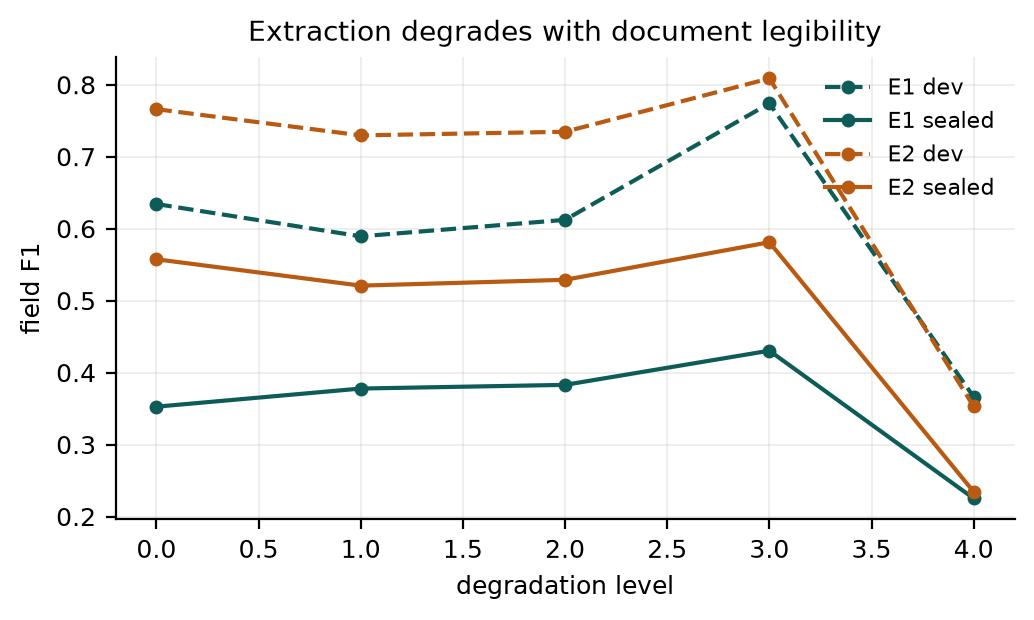
\includegraphics[width=0.9\linewidth]{../figures/fig05_extraction_by_degradation.png}
\caption{Extraction performance by layout degradation.}
\label{fig:extraction}
\end{figure}

\subsection{Reliability of the Extraction Signal}
\label{sec:reliability}

Raw OCR engine confidence and a small learned estimator (a gradient-boosted
classifier trained on extraction-level features) were compared as
predictors of whether an extracted clinical field was correct, evaluated on
sealed layouts.

\begin{table}[!t]
\caption{Reliability estimator comparison}
\label{tab:reliability}
\centering
\begin{tabular}{@{}llrrr@{}}
\toprule
Extractor & Signal & AUROC & Brier & ECE \\
\midrule
E1 & raw OCR conf. & 0.5214 & 0.2473 & 0.2254 \\
E1 & learned estimator & 0.9799 & 0.0542 & 0.0294 \\
E2 & raw OCR conf. & 0.6389 & 0.3806 & 0.3854 \\
E2 & learned estimator & 0.9871 & 0.0427 & 0.0151 \\
\bottomrule
\end{tabular}
\end{table}

Raw OCR confidence is close to chance-level for E1 and only modestly better
for E2 (Fig.~\ref{fig:reliability}) --- it measures how clearly the engine
read the text, not whether the resulting value is correct for its field.
The learned estimator's feature importances explain the gap: value
format-validity and value length dominate the decision (combined weight
$\approx0.86$), while raw OCR confidence contributes $\approx0.08$. A field
can be read with high OCR confidence and still be semantically wrong for
its slot, which is exactly the failure raw confidence cannot detect and a
format check can.

\begin{figure}[!t]
\centering
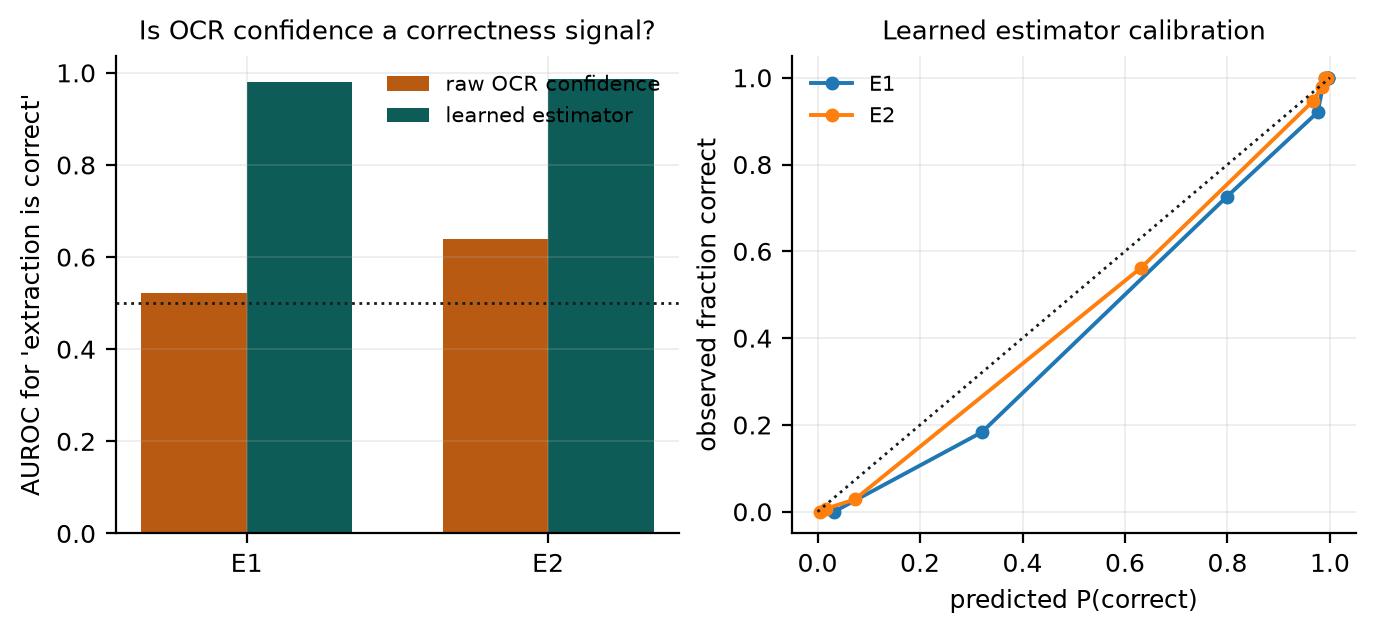
\includegraphics[width=0.9\linewidth]{../figures/fig06_reliability.png}
\caption{Raw OCR confidence vs.\ learned extraction-correctness estimator.}
\label{fig:reliability}
\end{figure}

\section{Triage}
\label{sec:triage}

\subsection{Deferral with Document Evidence}

The screening prototype answers with a predicted class whenever it chooses
to answer, and defers otherwise. Three systems were compared against an
image-confidence-only baseline: System~A, two hand-written rules combining
image confidence and document agreement; System~B, a learned gate that
additionally takes the extraction-reliability estimate $\hat{c}$
(Section~\ref{sec:reliability}) as input; and System~B without $\hat{c}$,
isolating that estimate's contribution. A falsification rule was fixed
before this experiment ran: if System~B did not outperform System~A, the
paper would present the rule-based system and report the learned gate as a
negative result.

\begin{table}[!t]
\caption{Deferral system comparison}
\label{tab:deferral}
\centering
\begin{tabular}{@{}lrrr@{}}
\toprule
System & AURC $\downarrow$ & Error-det.\ AUROC & Acc.@50\% \\
\midrule
Image conf.\ only & 0.3889 & 0.5875 & 0.5889 \\
\textbf{System A (rules)} & \textbf{0.1973} & \textbf{0.8817} & 0.8667 \\
System B (learned) & 0.2107 & 0.8692 & 0.8889 \\
System B w/o $\hat{c}$ & 0.2032 & 0.8705 & 0.8667 \\
\bottomrule
\end{tabular}
\end{table}

Document evidence produces a substantial improvement over image confidence
alone (Fig.~\ref{fig:riskcov}) --- AURC falls from 0.389 to approximately
0.20, and error-detection AUROC rises from 0.59 to 0.88. That improvement,
however, is delivered by the \textbf{hand-written rules}, not the learned
gate: System~B does not outperform System~A, and removing $\hat{c}$ from
System~B \emph{improves} it slightly rather than degrading it. Per the
pre-registered rule, this paper presents System~A as the deferral mechanism
and reports the learned gate as a negative result rather than a headline
contribution. $\hat{c}$ is not thereby shown to be useless --- it remains a
strong estimator of extraction \emph{correctness} on its own terms
(Section~\ref{sec:reliability}, AUROC 0.98--0.99) --- but it adds nothing
measurable to the deferral decision once image confidence and document
agreement are available. This comparison rests on 180 sealed-layout rows;
a $\approx$0.01 AURC gap between System~B variants is within the noise
that sample size implies, so the accurate statement is that the learned
gate did not demonstrate an improvement, not that the rules are proven
superior.

\begin{figure}[!t]
\centering
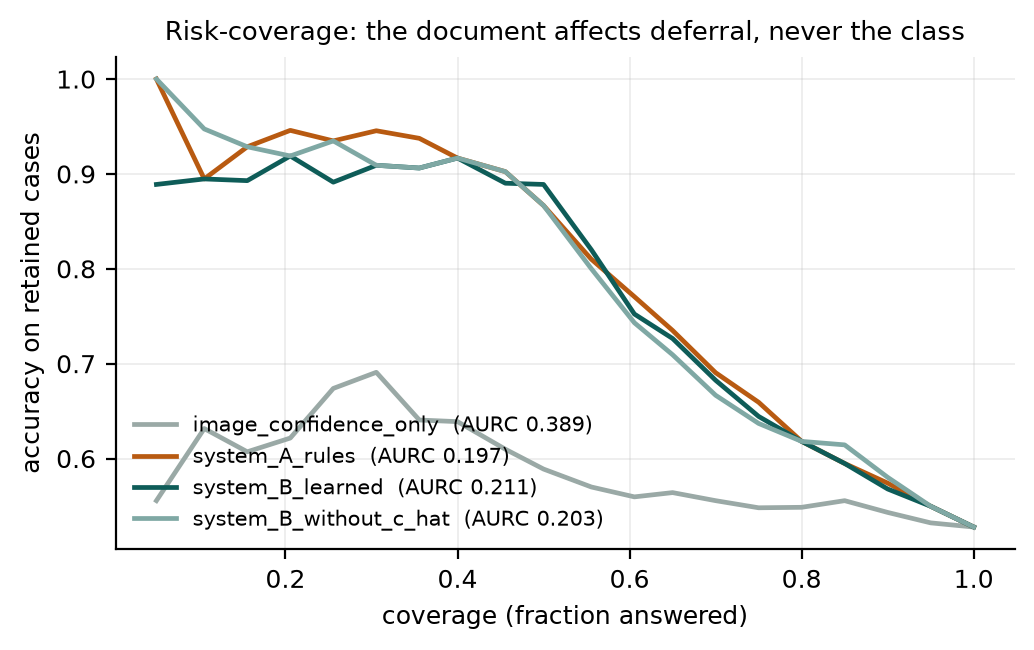
\includegraphics[width=0.9\linewidth]{../figures/fig07_risk_coverage.png}
\caption{Risk-coverage curves for all four deferral systems.}
\label{fig:riskcov}
\end{figure}

\subsection{Robustness Across Evidence Conditions}

A robustness matrix (Fig.~\ref{fig:robustness}) varies referral-document
quality and availability and confirms the deferral advantage from document
evidence persists across degraded-document conditions.

\begin{figure}[!t]
\centering
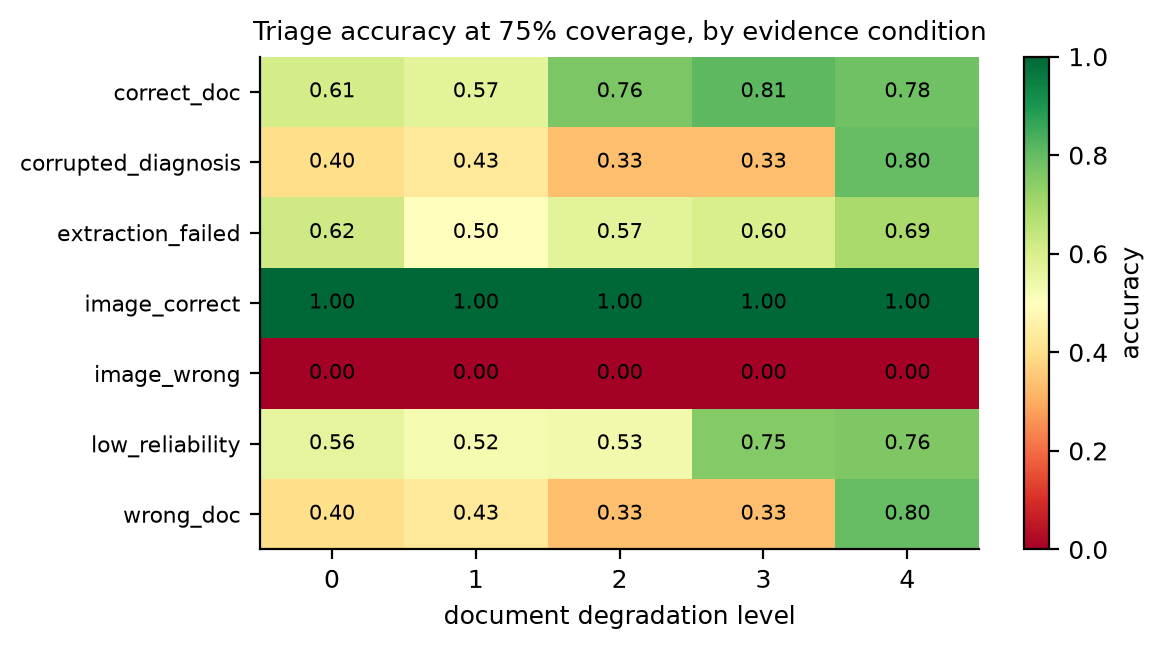
\includegraphics[width=0.9\linewidth]{../figures/fig08_robustness_matrix.png}
\caption{Deferral robustness across document-quality conditions.}
\label{fig:robustness}
\end{figure}

\subsection{Attribution}

Grad-CAM++, implemented via forward and backward hooks without an external
library dependency, was computed over the frozen-feature model on a
held-out fold the classification head had not been fitted on.

\begin{table}[!t]
\caption{Attribution summary}
\label{tab:attribution}
\centering
\begin{tabular}{@{}lr@{}}
\toprule
Measure & Value \\
\midrule
FOV-mass ratio (observed) & 0.8364 \\
Uniform-attribution baseline & 0.5348 \\
Concentration ratio & $1.56\times$ \\
Deletion AUC (mean) & 0.4687 \\
Randomization sanity check & pass ($r=-0.0943$) \\
\bottomrule
\end{tabular}
\end{table}

Attribution concentrates within the retinal field of view at 1.56$\times$
what uniform attention would produce (Fig.~\ref{fig:xai}), and the
randomization sanity check confirms the maps depend on the model's learned
weights rather than the attribution method's own structure. This licenses
the statement that attribution falls on retinal tissue rather than image
borders or letterboxing; it does not license any claim that the model
attends to a specific lesion, since no lesion masks and no ophthalmologist
review were available. Attribution here was computed on the frozen-feature
model rather than the fine-tuned model from Section~\ref{sec:results},
since Grad-CAM requires gradients through the backbone being evaluated, and
re-running this analysis on the fine-tuned backbone was not performed in
this iteration of the project.

\begin{figure}[!t]
\centering
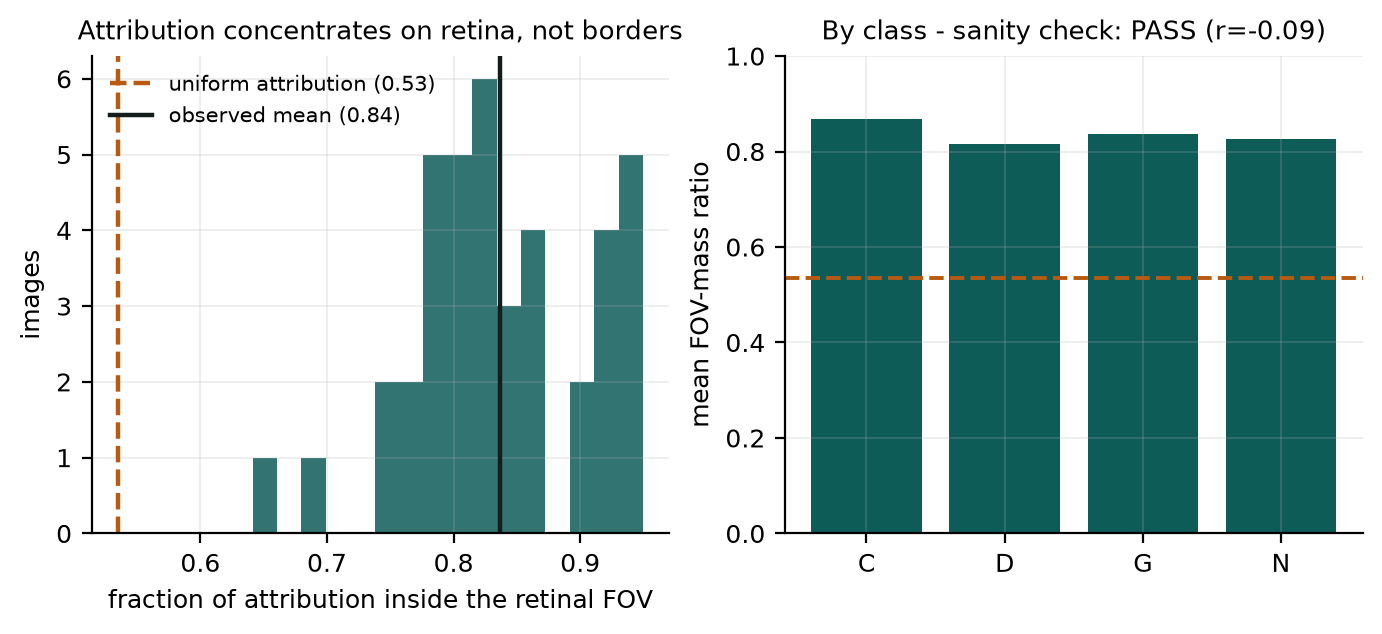
\includegraphics[width=0.9\linewidth]{../figures/fig12_xai.png}
\caption{Grad-CAM++ attribution and randomization sanity check.}
\label{fig:xai}
\end{figure}

\section{Limitations}

\begin{itemize}
\item Cataract and glaucoma classes contain 203 and 182 patients
  respectively. Findings involving these classes are reported as confidence
  intervals, not point estimates, and out-of-fold predictions are pooled
  before any significance test.
\item ODIR is less confounded than a naive multi-source merge, not
  confound-free: an $\approx$11-year age gap separates cataract and DR
  patients, sex distribution differs by class, and 23.2\% of
  glaucoma-labelled rows name a second condition.
\item The protocol-ladder result (Section~\ref{sec:results}) used a frozen
  linear head, which structurally cannot memorize. Section~\ref{sec:capacity}
  addresses this by sweeping model capacity, and the fine-tuned confirmation
  addresses it directly --- but every model in those sections still sits on
  frozen ImageNet features, and a differently fine-tuned backbone could
  behave differently again.
\item Attribution (Section~\ref{sec:triage}) is computed for the
  frozen-feature model, not the fine-tuned diagnostic model. It demonstrates
  attribution is concentrated on retinal tissue and passes a randomization
  sanity check; it does not demonstrate the model is examining a lesion.
\item The referral corpus is synthetic. Every derived number is a technical
  evaluation under controlled degradation, never a clinical validation. A
  search for a public, de-identified ophthalmic referral corpus is recorded
  rather than substituted with an unstated proxy.
\item The duplicate detector's recall is measured over ODIR$\leftrightarrow$
  merged-benchmark ground-truth pairs specifically; recall for duplicates
  occurring entirely within ODIR is not directly measurable with the ground
  truth available.
\item This work involves no prospective data collection, no clinical trial,
  and no regulatory clearance of any kind.
\end{itemize}

\section{Conclusion}

This paper set out to measure, rather than assume, how much of a widely
reported four-class ophthalmic screening benchmark's performance reflects
retinal pathology as opposed to how the benchmark was assembled.
Acquisition provenance was found to explain a substantial share of
separability, almost entirely for the diabetic-retinopathy and normal
classes and considerably less for cataract versus glaucoma. Patient-level
leakage produced no measurable effect on a low-capacity classifier but a
significant, monotonic effect that grows with model capacity, confirmed
directly on a fine-tuned deployable model rather than inferred from a
proxy. The trained classifier's apparent competence was shown not to rest
on the dataset's demographic confounds, and was shown not to transfer to
unseen acquisition sources. On the document-processing side, raw OCR
confidence was shown to be an unreliable signal of extraction correctness,
a learned alternative closed almost all of that gap, and a pre-registered
falsification rule led this paper to present hand-written deferral rules
rather than a more elaborate learned gate that did not, in fact, perform
better. Every finding above is reported with the model, sample size, and
statistical test that produced it, and every negative result --- the
initial leakage null, the failed embedding-based duplicate detector, the
learned deferral gate --- is reported as a negative result rather than
omitted.

\IEEEtriggeratref{3}
\begin{thebibliography}{00}

\bibitem{torralba2011} A. Torralba and A. A. Efros, ``Unbiased look at
dataset bias,'' in \emph{Proc. IEEE Conf. Computer Vision and Pattern
Recognition (CVPR)}, 2011, pp. 1521--1528.

\bibitem{liu2024decade} Z. Liu and K. He, ``A decade's battle on dataset
bias: Are we there yet?'' \emph{arXiv preprint arXiv:2403.08632}, 2024.

\bibitem{tampu2022} I. E. Tampu, A. Eklund, and N. Haj-Hosseini,
``Inflation of test accuracy due to data leakage in deep learning-based
classification of OCT images,'' \emph{Scientific Data}, vol. 9, 2022,
doi: 10.1038/s41597-022-01618-6.

\bibitem{leibig2017} C. Leibig, V. Allken, M. S. Ayhan, P. Berens, and S.
Wahl, ``Leveraging uncertainty information from deep neural networks for
disease detection,'' \emph{Scientific Reports}, vol. 7, no. 17816, 2017.

\bibitem{araujo2020} T. Ara\'ujo, G. Aresta, L. Mendon\c{c}a, S. Penas, C.
Maia, \^A. Carneiro, A. M. Mendon\c{c}a, and A. Campilho, ``DR$|$GRADUATE:
Uncertainty-aware deep learning-based diabetic retinopathy grading in eye
fundus images,'' \emph{Medical Image Analysis}, vol. 63, p. 101715, 2020.

\bibitem{zhang2023qmf} Q. Zhang, H. Wu, C. Zhang, Q. Hu, H. Fu, J. T. Zhou,
and X. Peng, ``Provable dynamic fusion for low-quality multimodal data,''
in \emph{Proc. Int. Conf. Machine Learning (ICML)}, 2023.

\bibitem{han2021tmc} Z. Han, C. Zhang, H. Fu, and J. T. Zhou, ``Trusted
multi-view classification,'' in \emph{Proc. Int. Conf. Learning
Representations (ICLR)}, 2021.

\bibitem{she2025multiretnet} J. She and K. Spivakovsky, ``MultiRetNet: A
multimodal vision model and deferral system for staging diabetic
retinopathy,'' \emph{arXiv preprint arXiv:2507.14738}, 2025.

\bibitem{yavari2026} A. Yavari, T. Schmoll, R. A. Leitgeb, K. L. Huber, H.
Stino, A. Pollreisz, W. Drexler, and T. Schlegl, ``Applicability study of
AI attribution methods for ophthalmic image classification,'' \emph{Scientific
Reports}, 2026, doi: 10.1038/s41598-025-33120-5.

\bibitem{simsa2023docile} \v{S}. \v{S}imsa, M. \v{S}ulc, M. U\v{r}i\v{c}\'a\v{r},
Y. Patel, A. Hamdi, M. Koci\'an, M. Skalick\'y, J. Matas, A. Doucet, M.
Coustaty, and D. Karatzas, ``DocILE benchmark for document information
localization and extraction,'' in \emph{Proc. Int. Conf. Document Analysis
and Recognition (ICDAR)}, 2023.

\end{thebibliography}

\end{document}
